\documentclass[handout]{beamer}
\usepackage[german]{babel}

\usepackage{fontspec} 
% \usepackage{lsp-makros}
\useoutertheme{lsp}

\usepackage{lsptitle}

\def\two@digits#1{\ifnum#1<10 0\fi\number#1}
\def\mytoday{\two@digits{\number\day}.\two@digits{\number\month}.\number\year}


\usepackage{xspace,multicol}
\newcommand{\latex}{\LaTeX\xspace}
\usepackage{tikz}


\newcounter{lastpagemainpart}
\footnotesep0pt
\renewcommand{\footnoterule}{}
\usefootnotetemplate{
  \noindent
  \insertfootnotemark\insertfootnotetext}

\let\beamerfn=\footnote
\renewcommand{\footnote}[1]{%
\let\oldfnsize=\footnotesize%
\let\footnotesize=\tiny%
\beamerfn<\thebeamerpauses$\to${#1}%
\let\footnotesize=\oldfnsize}


\date{\today}

\usepackage{eurosym}  
 
\renewcommand{\centerline}[1]{\hfill#1\hfill\hfill\mbox{}}


\title{\mbox{Platinum-Open-Access-Bücher} in der Sprachwissenschaft}
% \institute{FU Berlin}
\author[LangSci]{Sebastian Nordhoff}



\begin{document}
\lspbeamertitle


\section{Bücher}
\frame{
\frametitle{Bücher}
%   \includegraphics[height=.2\textheight]{./path/to/graphicsfile}
  \begin{itemize}
    \item Langform
    \begin{itemize}
      \item  Monographien
      \item Sammelbände
    \end{itemize}
    \item  eher nicht als HTML zu lesen
    \begin{itemize}
      \item pdf
      \item Papier
    \end{itemize}
    \item  längerer Publikationsprozess als bei Artikeln
    \begin{itemize}
      \item  Jahre bis Jahrzehnte Vorbereitung
    \end{itemize}
    \item weniger kommodifiziert als Artikel
  \end{itemize}
}

\section{Language Science Press}
\frame{
\frametitle{Language Science Press}
\begin{columns}
\column{6cm}
  \begin{itemize}
    \item gemeinnütziger Verlag in Wissenschaftshand
    \item 30 Reihen
    \item 695 Publikationsvoranfragen
    \item 180 Bücher seit 2014
    \begin{itemize}
      \item 30/Jahr
    \end{itemize}
    \item 76--1632 Seiten
    \item weltweite Autorenschaft
    \begin{itemize}
      \item Sydney, Yale, Hong Kong, Mexiko-Stadt, \dots
    \end{itemize}
    \item 1,5 Millionen Downloads
    \begin{itemize}
      \item max. pro Titel: 75.000 Downloads
    \end{itemize}
  \end{itemize}
  \column{4cm}
  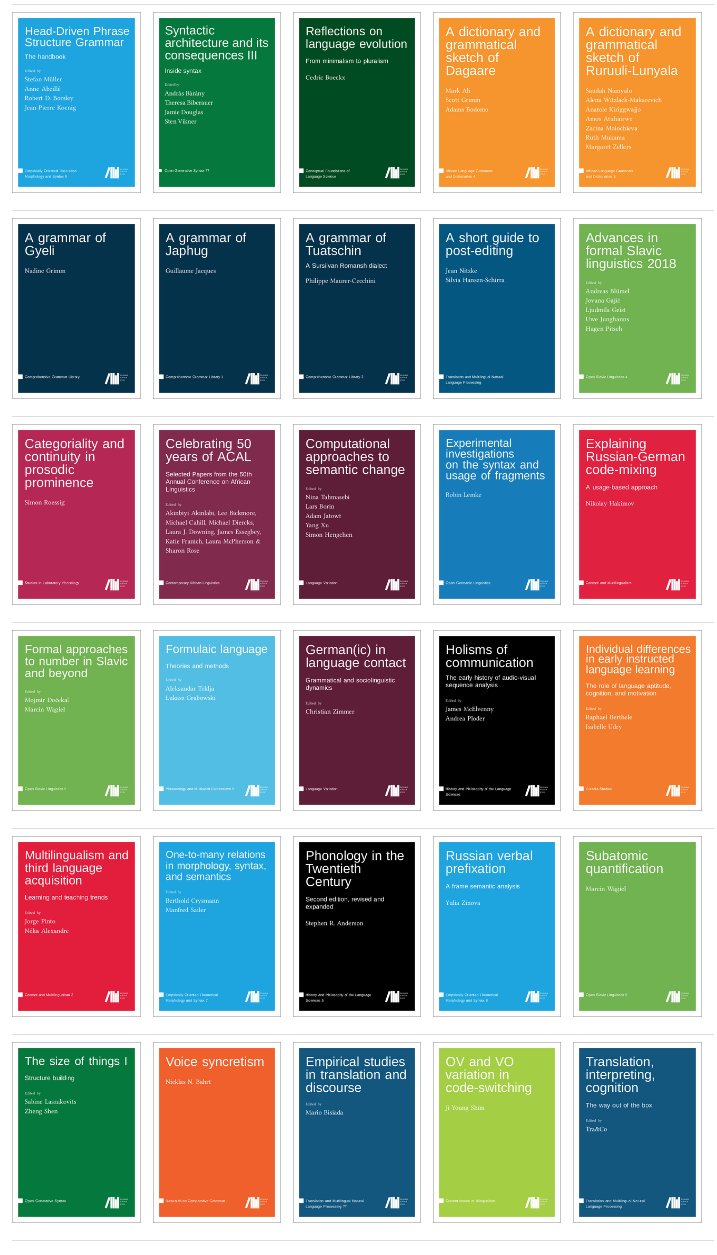
\includegraphics[height=\textheight]{output2022.png}
\end{columns}
}

\section{Finanzierungsmodelle}
\frame{
\frametitle{Finanzierungsmodelle}
%   \includegraphics[height=.2\textheight]{./path/to/graphicsfile}
Buchpublikation verursacht Kosten. Diese können auf verschiedenem Wege gegenfinanziert werden
  \begin{enumerate}
    \item   Reader-Pays
    \begin{itemize}
      \item Subskription
      \item Green OA
    \end{itemize}
    \item Author-Pays
    \begin{itemize}
      \item Autorinnengebühren
      \item Gold OA
    \end{itemize}
    \item Community-Pays
    \begin{itemize}
      \item Institutionelle Unterstützer
      \item Diamond/Platinum OA
    \end{itemize}
  \end{enumerate}
}

\frame{
\frametitle{Probleme der Finanzierungsmodelle}
  \begin{itemize}
    \item  \textbf{reader-pays: serials crisis}
    \begin{itemize}
      \item Preise für Zeitschriften-Abos steigen überdurchschnittlich
      \begin{itemize}
        \item Produktionskosten für Artikel allerdings vergleichbar
        \item 30\% Umsatzrendite der großen Verlage
      \end{itemize}
    \end{itemize}
    \item \textbf{author-pays: APC crisis (Elio Pellin)}
    \begin{itemize}
      \item Autorengebühren steigen überdurchschnittlich
      \begin{itemize}
        \item Produktionskosten für Artikel allerdings vergleichbar
        \item 30\% Umsatzrendite der großen Verlage
      \end{itemize}
    \end{itemize}
    \item Wert bemisst sich nach Prestige
    \begin{itemize}
        \item Jedes Mal, wenn Sie in der Pizzeria Cavalli essen, wird die Pizza 1 CHF teurer.
    \end{itemize}
  \end{itemize}
  \centering 
\includegraphics[height=.4\textheight]{cavalli.png}
}


\frame{
\frametitle{Pizzeria Cavalli}
\includegraphics[height=\textheight]{mapcavalli.png}
}


\frame{
\frametitle{Röthlisberger}
\includegraphics[height=\textheight]{menti.png}
}

\frame{
\frametitle{Fonds UB Bern}
\includegraphics[height=\textheight]{pellin.png}
}


\frame{
\frametitle{€€ \$\$ ££}
 
\includegraphics[height=\textheight]{cavalli.png}
}




\frame{
\frametitle{Lösung}
%   \includegraphics[height=.2\textheight]{./path/to/graphicsfile}
  \begin{itemize}
    \item   Marken in Wissenschaftshand
    \item  \textbf{Die Marke \textit{Language Science Press} gehört einer gemeinnützigen Gesellschaft und kann nicht verkauft werden}
    \item Gewinnausschüttung ist gesetzlich untersagt
    \item alle Erlöse müssen für Förderung von Wissenschaft und Forschung (+Volksbildung) eingesetzt werden
    \begin{itemize}
      \item keine Dividenden o.ä.
    \end{itemize}
    \item $\to$ keine Veranlassung, mehr Geld zu nehmen als für den Betrieb notwendig
  \end{itemize}
}

\frame{
\frametitle{Geldströme}
%   \includegraphics[height=.2\textheight]{./path/to/graphicsfile}
  \begin{itemize}
    \item \parbox{25mm}{\textbf{Green OA}:}\\  \fbox{Steuerzahler\strut} $\to$ UB $\to$ Erwerbungsbudget $\to$ \fbox{Verlag\strut}
    \item \parbox{25mm}{\textbf{Gold OA}:}\\  \fbox{Steuerzahler\strut} $\to$ UB $\to$ OA-Fonds $\to$ APCs $\to$ \fbox{Verlag\strut}
    \item \parbox{25mm}{\textbf{Diamond OA}:}\\  \fbox{Steuerzahler\strut} $\to$ UB $\to$ OA-Fonds $\to$ Mitgliedschaft $\to$ \fbox{Verlag\strut}

%       \begin{itemize}
%         \item KOALA-Projekt an der TIB Hannover \url{https://projects.tib.eu/koala}
%         \item \textbf{K}onsortiale \textbf{OA}-\textbf{L}ösungen \textbf{A}ufbauen.
%       \end{itemize}
  \end{itemize}
}

\section{Setup}
\frame{
\frametitle{Setup}
%   \includegraphics[height=.2\textheight]{./path/to/graphicsfile}
  \begin{itemize}
    \item  116 Unterstützerorganisationen weltweit
    \begin{itemize}
      \item Basel, Bern, Lausanne,  Neuenburg, Zürich
    \end{itemize}

    \item  1000 €/Jahr
    \item  davon werden produziert: 30 Bücher
    \item  wenn Geld  übrig bleibt
    \begin{itemize}
      \item     mehr Bücher
    \end{itemize}
    \item Finanzierungsrunden (Knowledge Unlatched)
    \begin{itemize}
      \item  2018-2020 (erfolgreich abgeschlossen, 94 Bücher)
      \item  2021-2023 (laufend, bisher 35 Bücher)
    \end{itemize}
  \end{itemize}
}

\frame{
\frametitle{Buchproduktion und -vertrieb}
%   \includegraphics[height=.2\textheight]{./path/to/graphicsfile}
\begin{columns}
\column{7cm}
  \begin{itemize}
    \item kollaborative und versionierte Dokumentenerstellung
    \begin{itemize}
    \item  \LaTeX{} mit Overleaf
    \item git zur Versionierung
    \item PaperHive zur Kommentierung
    \item Zenodo zur Archivierung
    \item Vertrieb über Print-on-Demand
    \item OAPEN/DOAB, VLB, GoogleBooks, Amazon
    \end{itemize}
  \end{itemize}
\column{3cm}\hspace*{-1.8cm}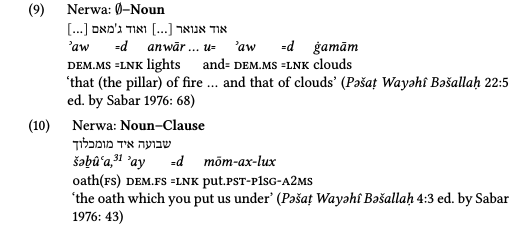
\includegraphics[height=.37\textheight]{nena.png}

~ \hspace{2cm} ~
\end{columns}
}


\section{Werte}

\frame{
\frametitle{Werte}
\begin{columns}
\column{3cm}
  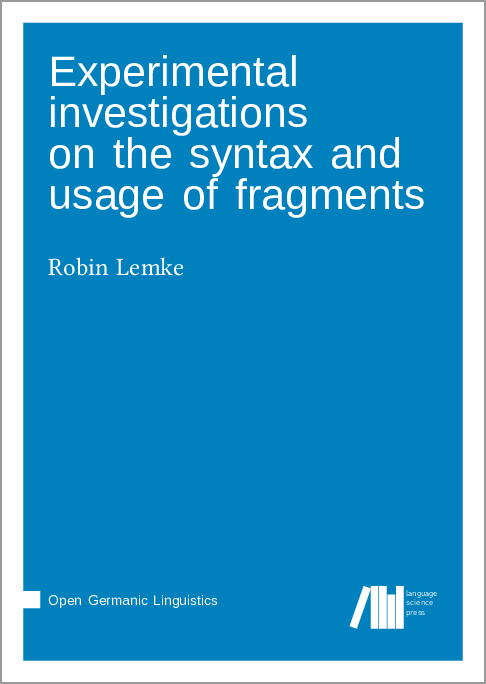
\includegraphics[height=.4\textheight]{lemke.png}
\includegraphics[height=.4\textheight]{easterday.png}
  
\includegraphics[height=.4\textheight]{roessig.png}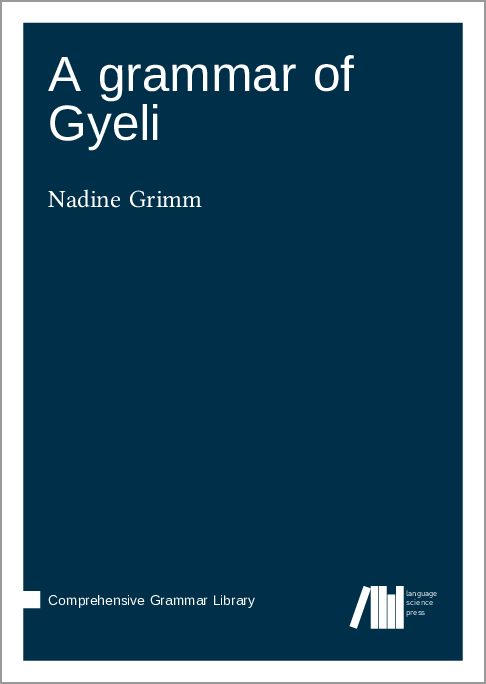
\includegraphics[height=.4\textheight]{gyeli.png}
\column{7cm}
  \begin{enumerate}
    \item \textbf{Exzellenz}
    \begin{itemize}
      \item strikte Qualitätskontrolle
      \item diverse Preise und Auszeichnungen
    \end{itemize}
    \item \textbf{Transparenz}
    \begin{itemize}
      \item Open Access
      \begin{itemize}
        \item incl. Quellcode, Rohdaten und record of versions
      \end{itemize}
      \item Open Source
      \begin{itemize}
        \item CTAN, PyPI, GitHub
    \end{itemize}
      \item Open Data
      \item Open Bookkeeping
    \end{itemize}
    \item \textbf{Community}
    \begin{itemize}
      \item 1200 Unterstützerinnen
      \item 500 Mitglieder Editorial Boards
      \item 500 Community Proofreader
    \end{itemize}
  \end{enumerate}
\end{columns}
}


\frame{
\frametitle{Vorteile}
%   \includegraphics[height=.2\textheight]{./path/to/graphicsfile}
  \begin{enumerate}
    \item  effizienter Mitteleinsatz
    \begin{itemize}
      \item Kosten pro Buch ca. 4000€ vgl. mit 10-20.000 bei kommerziellen Verlagen
    \end{itemize}
    \item  autonome Reihen
    \item  gute Verbreitung
    \item Autorinnen behalten Copyright
    \item keine Geldabschöpfung
    \item  ``gerechter''
  \end{enumerate}
}

\frame{
\frametitle{Nachteile}
%   \includegraphics[height=.2\textheight]{./path/to/graphicsfile}
  \begin{enumerate}
    \item Wachstum nur in 3-Jahres-Intervallen möglich.
    \item Derzeit keine Abdeckung aller Teilgebiete der Sprachwissenschaft, z.B. Semantik
  \end{enumerate}
}


\section{Ausblick}

\frame{
\frametitle{Ausblick: Warum machen wir das eigentlich?}
%   \includegraphics[height=.2\textheight]{./path/to/graphicsfile}
  \begin{itemize}
    \item  Macht Open Access im allgemeinen \ldots
    \begin{itemize}
      \item {\ldots} Wissen zugänglicher?
      \item {\ldots} Wissensvermittlung preiswerter?
      \item {\ldots} Wissensproduktion demokratischer?
    \end{itemize}
    \item Die Antworten sind für Grün/Gold/Platin unterschiedlich.
  \end{itemize}
}

\frame{
\frametitle{Ausblick:\\Community vs.\ Region}
%   \includegraphics[height=.2\textheight]{./path/to/graphicsfile}
  \begin{itemize}
    \item Wissenschaft ist in weltweiten Communitys organisiert
    \item Die Berner Chemikerin hat mehr mit der Chemikerin in Shanghai gemein als mit dem Berner Theologen.
    \item Erfolgreiche OA-Projekte sind disziplinär organisiert, nicht regional
    \begin{itemize}
      \item Hochenergiephysik (SCOAP³), Linguistik, Geologie (Copernicus)
    \end{itemize}
  \end{itemize}
}

\frame{
\frametitle{Disziplinäre Netzwerke}
  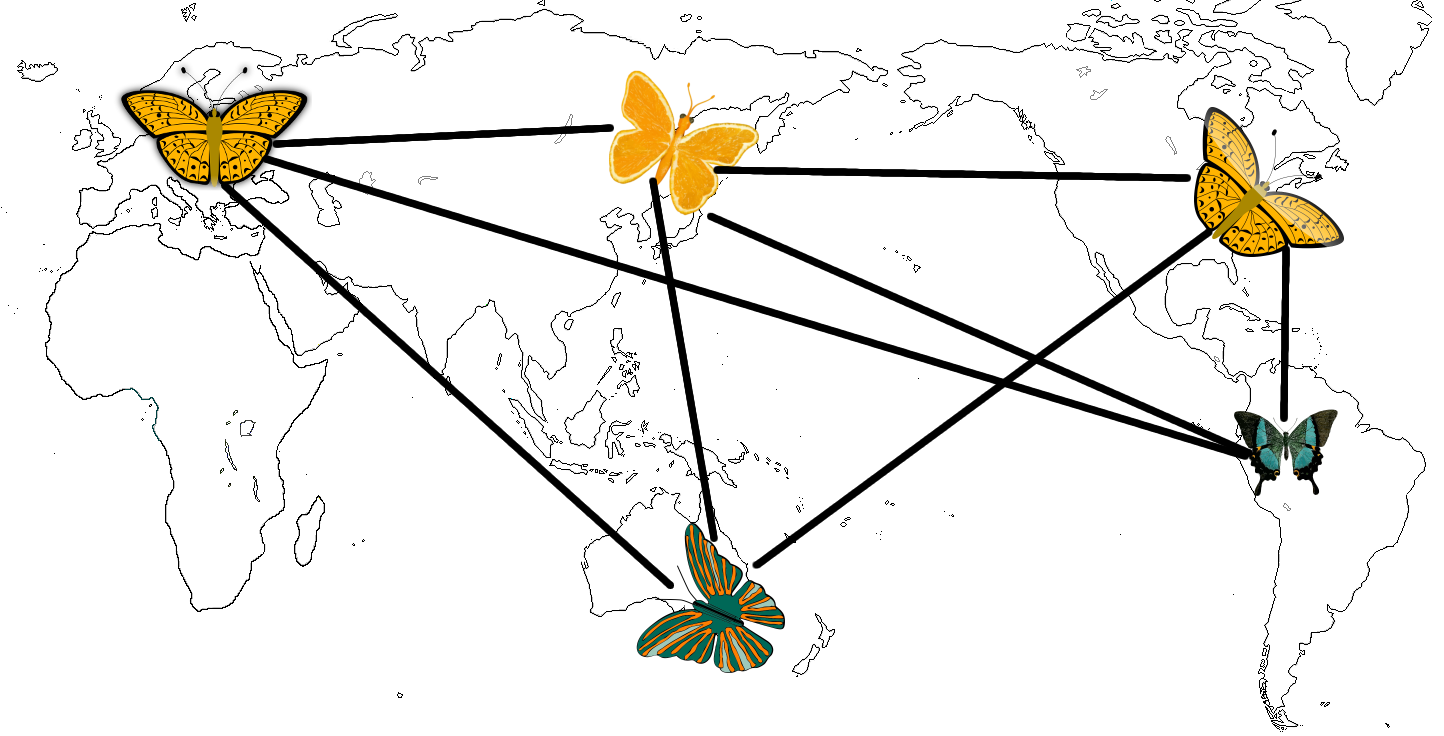
\includegraphics[height=\textheight]{schmetterlinge.png}
}

\frame{
\frametitle{Disziplinäre Netzwerke}
  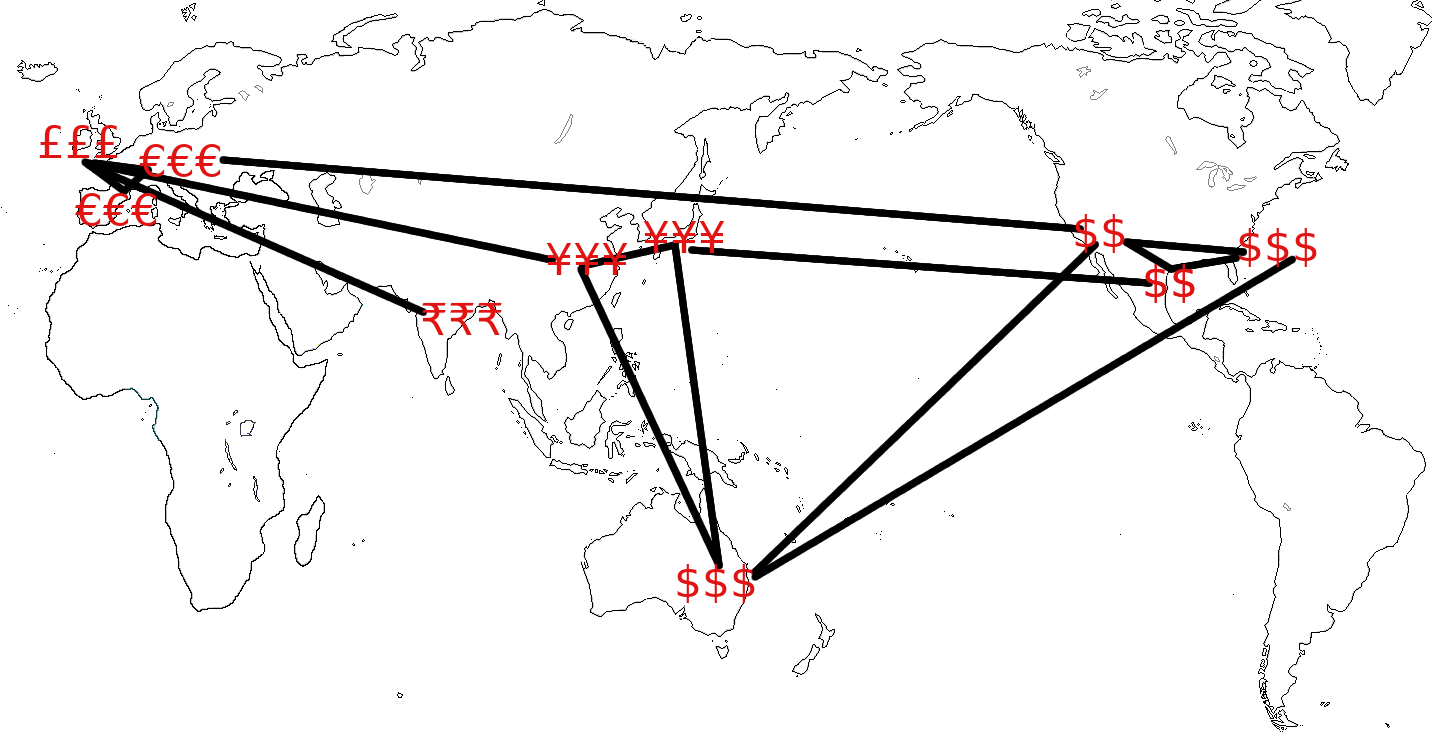
\includegraphics[height=\textheight]{geld.png}
}

\frame{
\frametitle{Disziplinäre Netzwerke}
  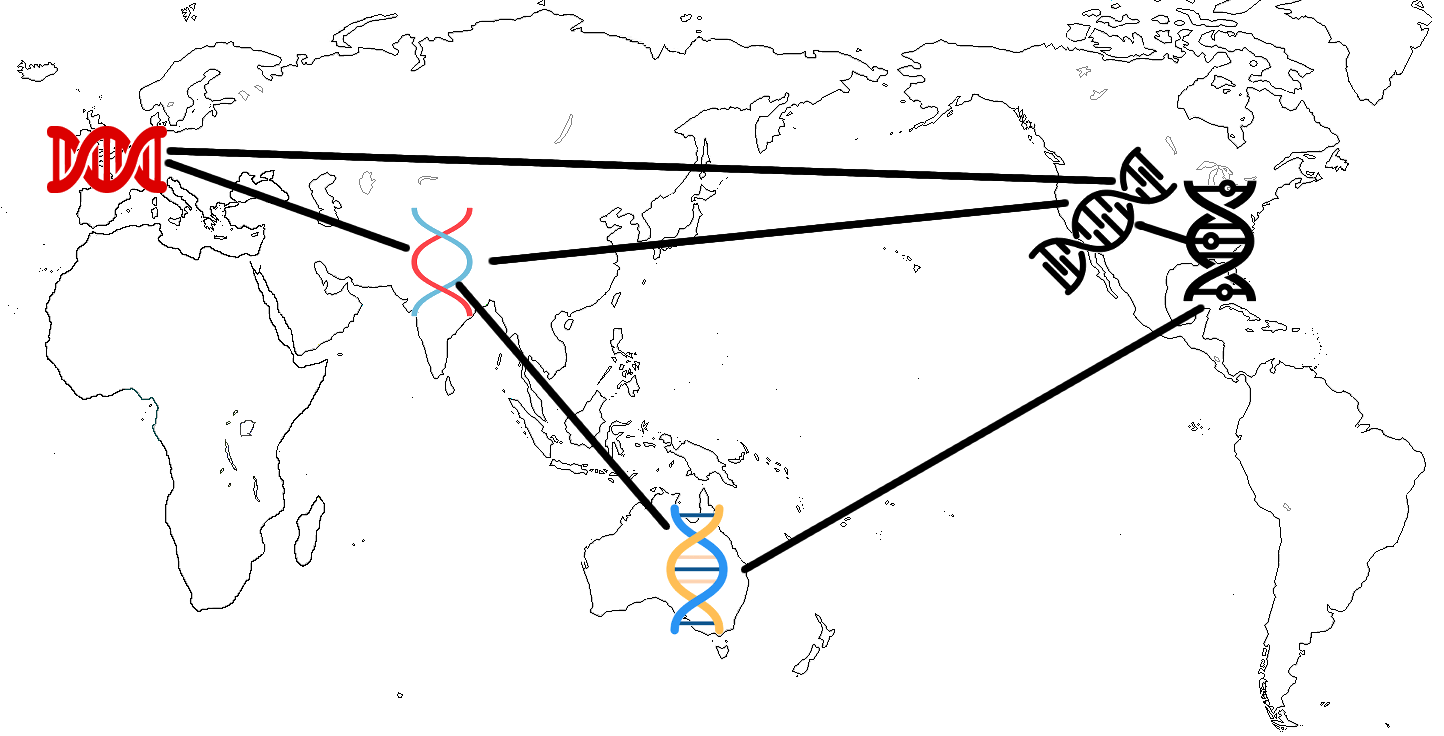
\includegraphics[height=\textheight]{viren.png}
}

\frame{
\frametitle{Regionale Netzwerke}
  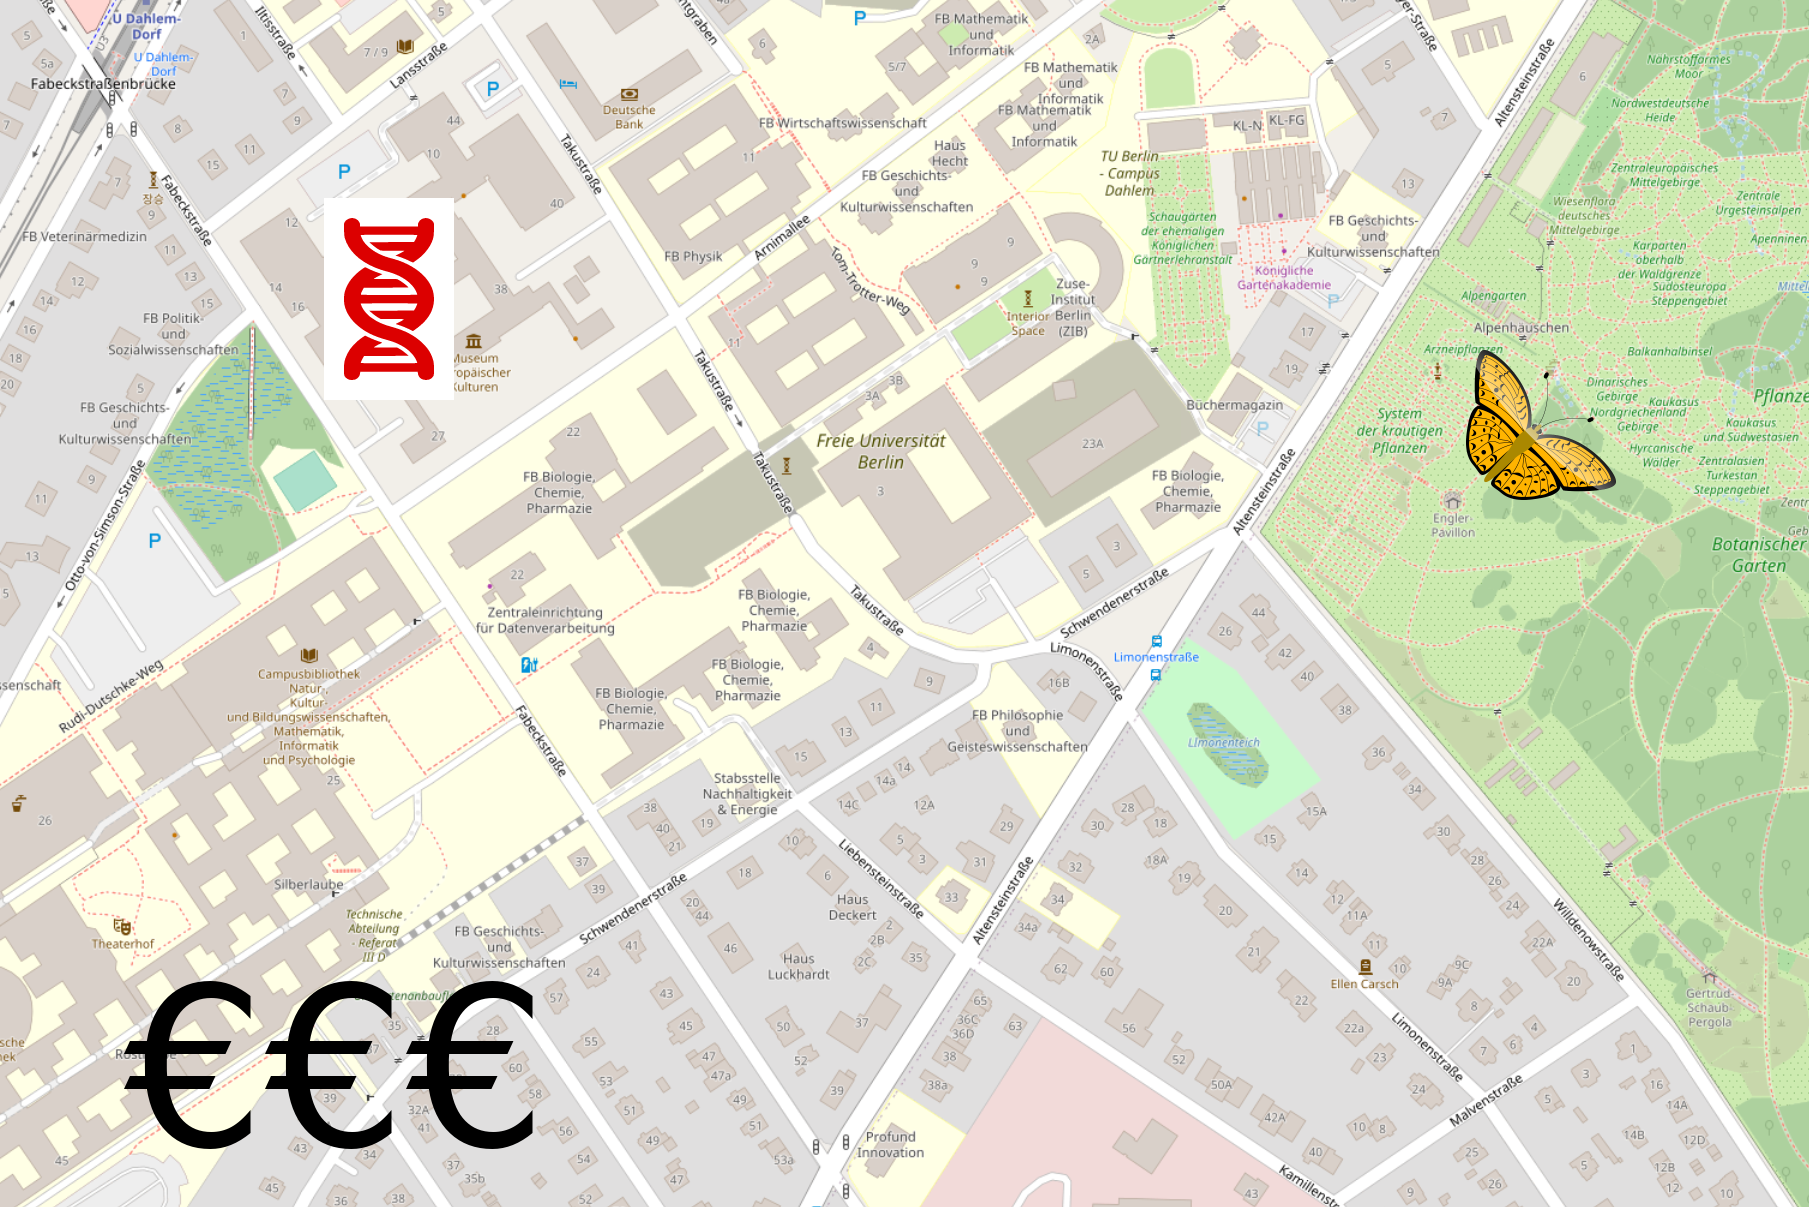
\includegraphics[height=\textheight]{universitaetsverlag.png}
}


\frame{
\frametitle{Vielen Dank}
\hspace*{-1cm}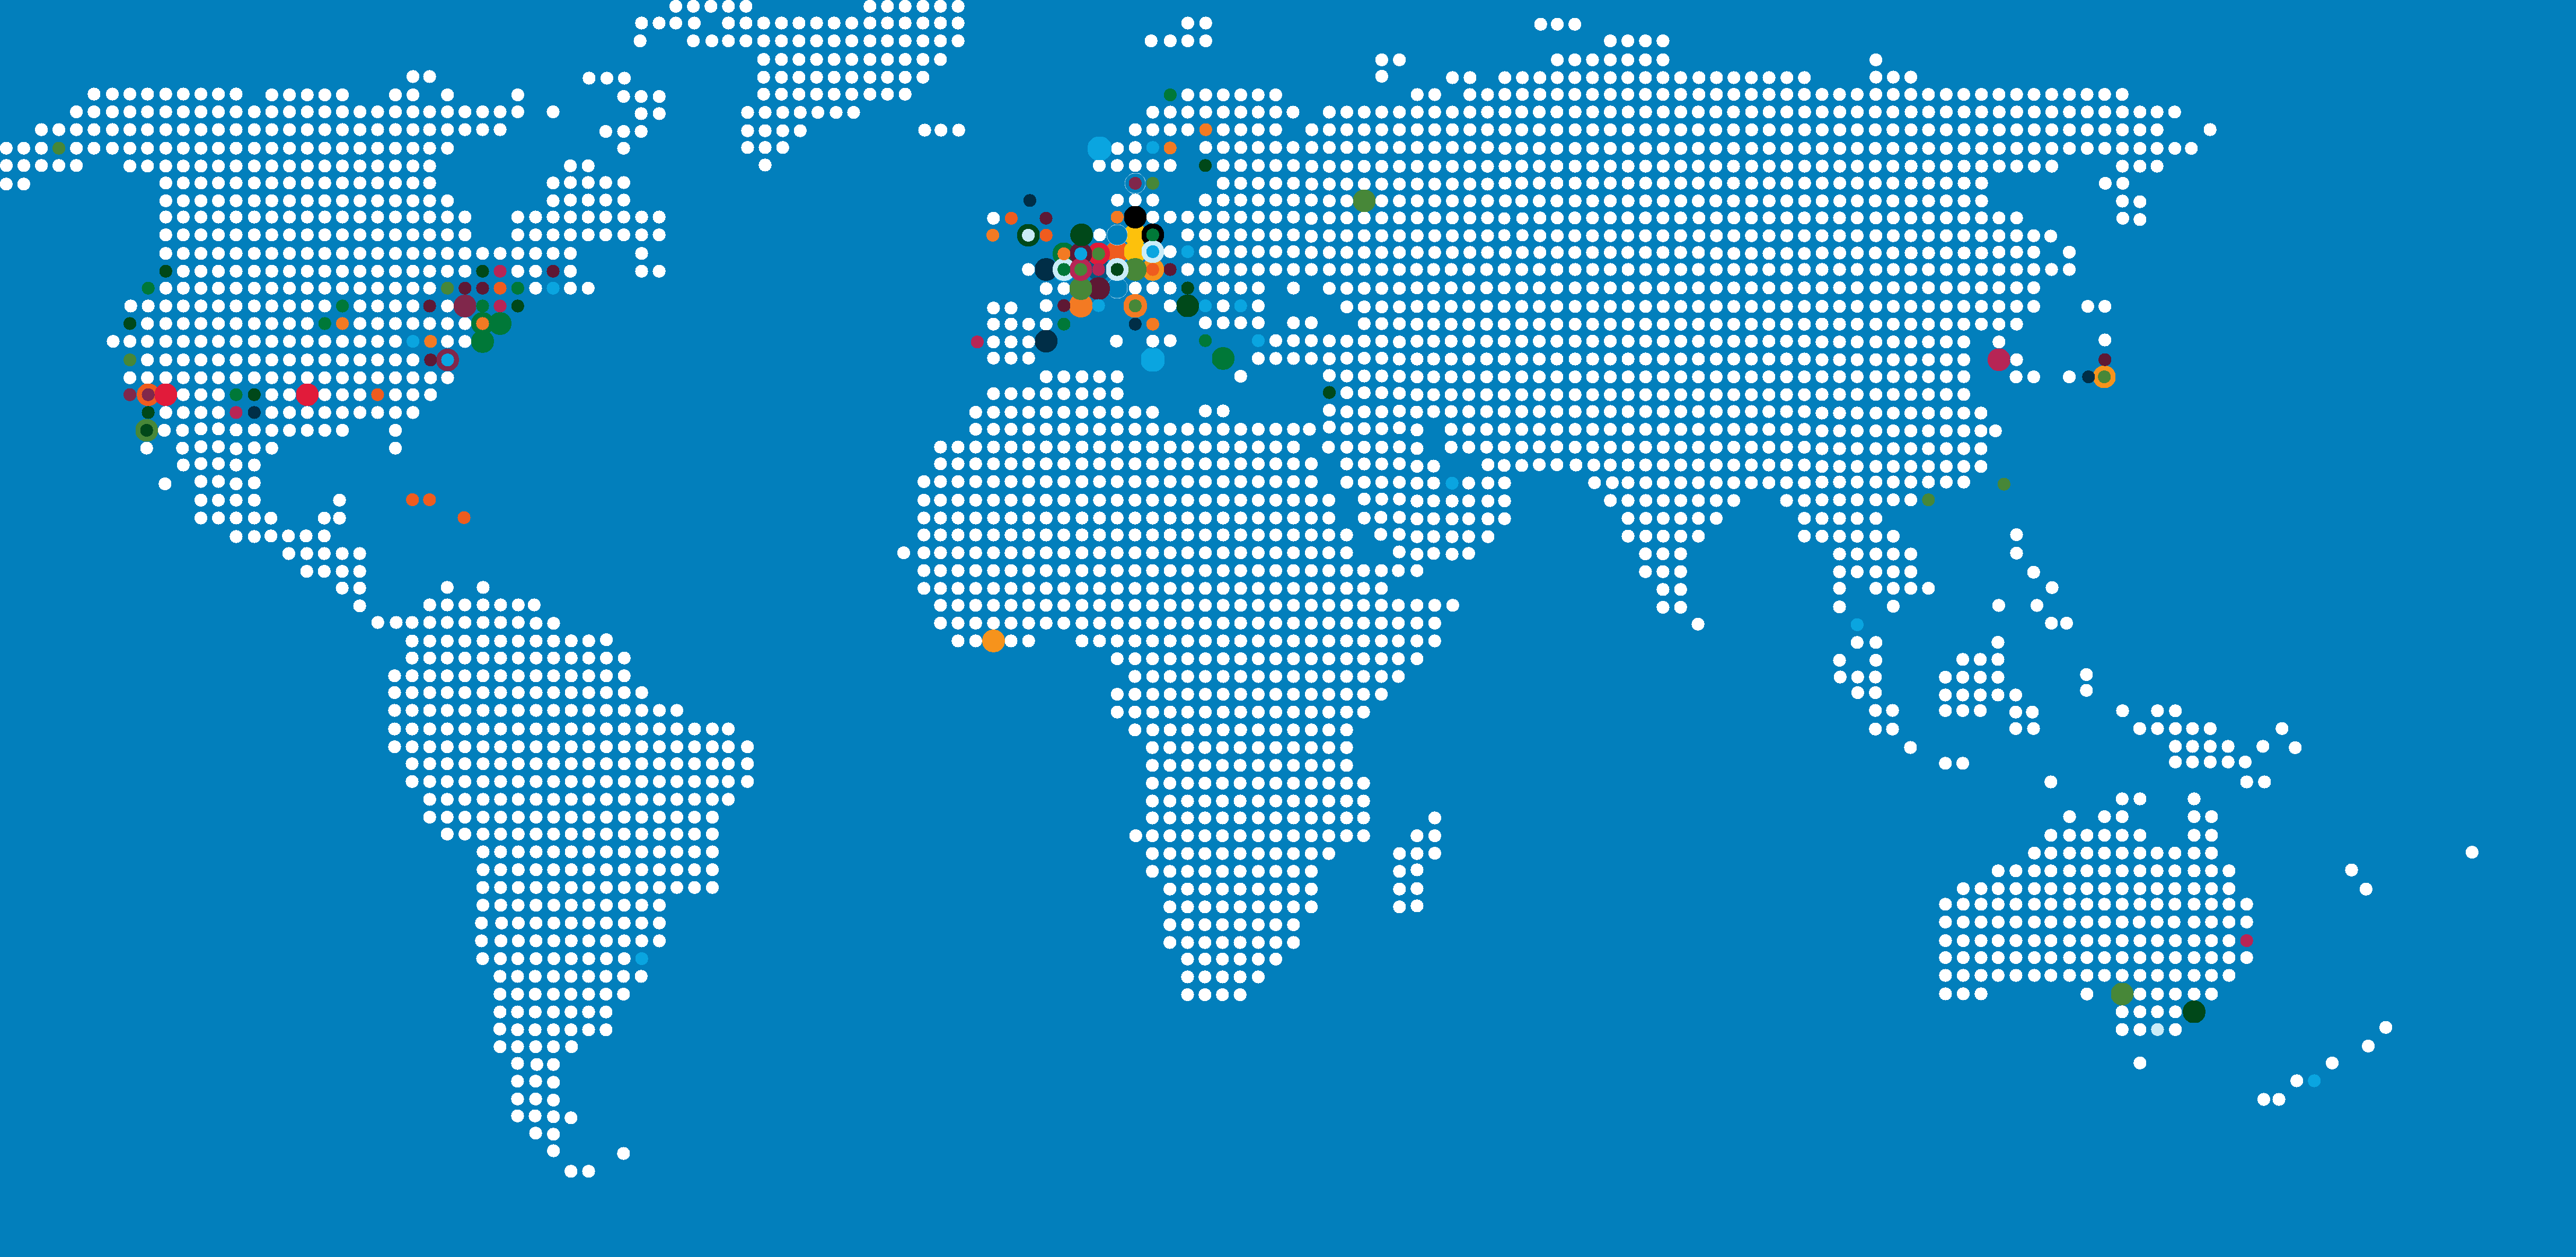
\includegraphics[height=\textheight]{WORLDMAPDOTSdots.png}
}

\frame{
\frametitle{Lizenz}
Lizenziert unter CC-BY 4.0 https://creativecommons.org/licenses/by/4.0/
}

%\setcounter{framenumber}{\thelastpagemainpart}
\end{document}
